\documentclass[11pt]{article}

\usepackage[margin=1in]{geometry}
\usepackage{amsmath,amssymb,amsthm}
\usepackage{graphicx}
\usepackage{booktabs}
\usepackage{multirow}
\usepackage{microtype}
\usepackage{xcolor}
\usepackage[colorlinks=true,linkcolor=blue!60!black,citecolor=blue!60!black,urlcolor=blue!60!black]{hyperref}
\usepackage[numbers,sort&compress]{natbib}
\usepackage{algorithm}
\usepackage{algpseudocode}
\usepackage{caption}
\captionsetup{font=small,labelfont=bf}

\newcommand{\facet}{\textsc{Facet}}
\newcommand{\hproxy}{$H_{\text{proxy}}$}
\newcommand{\ppobc}{PPO\textsubscript{BC}}

\newcommand{\repourl}{https://github.com/aarushkandukoori/facet}

\title{\textbf{\facet{}: Prioritized Population-Based Reinforcement Learning\\
for Human-Compatible Multiplayer Agents}}

\author{%
  Aditya Kandukoori\thanks{Jewel Labs Research --- \url{https://jewellabs.org}.} \\
  Poolesville High School
  \and
  Aarush Kandukoori\footnotemark[1] \\
  Carnegie Mellon University
  \and
  Soham Jariwala\footnotemark[1] \\
  Cornell University
  \and
  Khandaker Wasi\footnotemark[1] \\
  Cornell University
}
\date{August 2026}

\begin{document}
\maketitle

\begin{abstract}
AI agents are increasingly deployed in \emph{multiplayer workspaces}: shared
environments in which several agents and several humans act concurrently
toward a common objective, as in Jewel Labs' agentic infrastructure for the
diamond and jewelry trade. Reinforcement-learning agents trained by self-play
excel when paired with copies of themselves but are known to fail when paired
with partners---human or artificial---whose conventions differ from their own.
We present \facet{} (Fictitious Agent Co-training for Emergent Teamwork), a
lightweight population-based training method that (i) seeds the partner
population with behavior-cloned human models fit to real human gameplay,
(ii) adds frozen self-play checkpoints spanning multiple skill stages, and
(iii) prioritizes sampling toward the partners with which the learner
currently coordinates \emph{worst}. On the Overcooked-AI benchmark, using the
2019 human--human dataset (103{,}141 timesteps across five layouts), we train
and evaluate 75 models: behavior cloning (BC), self-play PPO (SP), PPO
trained with a fixed human model (\ppobc{}), and \facet{} (three seeds
each per layout), plus 15 held-out human-proxy models---and evaluate every
agent along two axes of the workspace problem: coordination with
\emph{held-out human proxies} and with an \emph{existing fleet} of
independently trained agents (in-distribution for \facet{} by
construction, unseen for the baselines). The classic failure reproduces
sharply at laptop scale: self-play loses 53--96\% of its self-paired score
when moved to human proxies. No single method dominates both
axes---\ppobc{} is the strongest human-proxy method (best of the four
methods on 3/5 layouts) but sacrifices fleet compatibility, while
self-play shows the reverse profile. Across the ten seed-averaged
(layout $\times$ partner-type) evaluation cells, \facet{} is the only
method without a catastrophic cell: its worst cell scores 12.7 versus
3.7--5.8 for all baselines, and it attains the best combined human+fleet
score under equal axis weighting (110.3 vs.\ 102.0 for \ppobc{} and 95.0
for SP; Section~6 discusses both qualifications). All code, all 75
trained models, and an interactive browser demo are
released.\footnote{\url{https://github.com/aarushkandukoori/facet}}
\end{abstract}

\section{Introduction}
\label{sec:intro}

Enterprise software is shifting from single-user tools to \emph{multiplayer
workspaces}: shared, real-time environments in which human teams and
autonomous AI agents act concurrently---humans monitoring, redirecting, and
approving while agents quote, plan, and verify. Jewel Labs' production
platform for the diamond trade is one such workspace: quoting, cut-planning,
and compliance agents operate alongside human traders in a shared operational
surface. In such settings the value of an agent is not its solo competence
but its \emph{team} competence: the joint performance of the human--agent
system~\citep{nationalacademies2022humanaiteaming}. This echoes a
25-year-old lesson from mixed-initiative interaction design---automation is
useful exactly insofar as it couples smoothly with human
activity~\citep{horvitz1999mixedinitiative}.

Reinforcement learning offers a direct way to train agents for interactive
multi-step tasks, and \emph{self-play}---training an agent with copies of
itself---is its workhorse. But a well-replicated finding in cooperative
multi-agent RL is that self-play agents develop private conventions that
shatter when the partner deviates from them. \citet{carroll2019utility}
demonstrated this on Overcooked, a two-player common-payoff cooking game:
agents trained by self-play or population-based training scored highly with
themselves yet often dropped below a simple imitation baseline when paired
with human proxies. \citet{hu2020otherplay} formalized the underlying issue as
\emph{zero-shot coordination} (ZSC): converging to arbitrary symmetric
conventions is optimal in self-play and catastrophic with novel partners.

Two families of remedies exist. \emph{Human-data} methods embed a learned
human model in training: \citet{carroll2019utility}'s \ppobc{} trains a best
response to a behavior-cloned human. \emph{Population} methods avoid human
data by training a best response to a diverse population: TrajeDi
originated the diversity-regularized population plus common-best-response
recipe~\citep{lupu2021trajectory}; Fictitious Co-Play (FCP)
\citep{strouse2021collaborating} showed that independent self-play runs
\emph{and their past checkpoints} suffice as partners; later work refines
the population via entropy bonuses~\citep{zhao2023maximum},
hidden-utility biases~\citep{yu2023hsp}, or generative partner
models~\citep{liang2024gamma}.

These two families are usually studied in opposition---with human data or
without. In a deployed multiplayer workspace, however, both resources exist
simultaneously: logs of real human behavior \emph{and} cheap self-play
checkpoints. \facet{} combines them. The partner population contains
behavior-cloned human models (convention anchors from real data) and frozen
self-play checkpoints from independent runs at four skill stages (cheap
convention and skill diversity, as in FCP). Training then applies a
\emph{prioritized sampling} rule inspired by MEP's second
stage~\citep{zhao2023maximum}: partners are drawn with probability increasing
in the learner's current \emph{failure} to coordinate with them, estimated by
an exponential moving average of episode returns. The learner therefore
spends its samples where its coordination is weakest---typically the human
models and the low-skill checkpoints---while never fully abandoning strong
partners.

We make three contributions:
\begin{enumerate}
  \item \textbf{Method.} \facet{}, a simple best-response-to-population
  scheme unifying human behavior models and self-play checkpoints under
  worst-partner-prioritized sampling (Section~\ref{sec:method}).
  \item \textbf{Controlled two-axis study at laptop scale.} A complete,
  reproducible comparison of BC, SP, \ppobc{}, and \facet{}---60 RL/imitation
  policies plus 15 held-out human-proxy models---trained on a single Apple
  M4 laptop in under six hours total, on all five layouts of the classic
  Overcooked human--human dataset~\citep{carroll2019utility}, and evaluated
  against both held-out human proxies and an existing agent fleet
  (Section~\ref{sec:setup}). All numbers in this paper are measured from
  these runs; no results are imported from prior work.
  \item \textbf{Open release.} Training code, all 75 model checkpoints,
  evaluation data, and an interactive in-browser replay demo of the trained
  agents.\footnote{\url{https://github.com/aarushkandukoori/facet}}
\end{enumerate}

Our headline results (Tables~\ref{tab:main} and~\ref{tab:fleet}): the
self-play failure reproduces dramatically---SP loses between 53\%
(Cramped Room) and 96\% (Forced Coordination) of its self-paired score when
paired with held-out human proxies. \ppobc{} is the strongest single-axis
human-compatibility method (its mean exceeds \facet{}'s on four of five
layouts on that axis), but it pays for that specialization on the
machine-partner axis, where \facet{}'s mean exceeds \ppobc{}'s on all five
layouts---an axis that is in-distribution for \facet{} by construction,
since its training pool contains the fleet runs' checkpoints
(Section~\ref{sec:setup}). No method wins everywhere; what the
multiplayer-workspace setting arguably demands is the \emph{absence of
catastrophic cells}, and on seed-averaged cells \facet{} is alone: its
worst of the ten (layout $\times$ partner-type) cell means is 12.7,
versus 3.7 for SP, 5.3 for \ppobc{}, and 5.8 for BC, and its combined
human+fleet average (110.3, equal axis weighting) is the highest of the
four methods. Individual seeds still fail---we report per-seed minima and
self-pairing deadlocks for \emph{all} methods, including \facet{}, in
Section~\ref{sec:results}.

\section{Related Work}
\label{sec:related}

\paragraph{Overcooked and human-compatible RL.}
\citet{carroll2019utility} introduced the two-player Overcooked benchmark,
collected the human--human dataset we use, and showed that self-play PPO and
population-based training degrade sharply when paired with human proxies
while \ppobc{} (best response to a behavior-cloned human) transfers better;
their user study (N=60) confirmed the effect with real humans. The benchmark
has since become the standard testbed for human--AI coordination. Follow-up
work has questioned aspects of its evaluation: ZSC-Eval~\citep{wang2024zsceval}
proposes best-response-diversity-based partner selection, and
OvercookedV2~\citep{gessler2025overcookedv2} argues the original layouts
under-test ZSC because broad state coverage suffices; we therefore report
per-layout results and self-pair/cross-pair gaps rather than a single
aggregate.

\paragraph{Population-based zero-shot coordination.}
Other-Play~\citep{hu2020otherplay} framed ZSC and showed self-play converges
to arbitrary conventions. TrajeDi~\citep{lupu2021trajectory} introduced the
diversity-regularized population plus common-best-response recipe; FCP
\citep{strouse2021collaborating} showed a population of self-play runs
\emph{and their checkpoints} suffices to coordinate with humans without human
data; MEP~\citep{zhao2023maximum} added a population-entropy bonus and
\emph{prioritized} partner sampling; HSP~\citep{yu2023hsp} argued populations
should span human \emph{biases}, not just skill; E3T~\citep{yan2023e3t}
questioned the cost of populations altogether; GAMMA~\citep{liang2024gamma}
replaced the discrete population with a generative partner model, optionally
biased by a small amount of human data. PECAN~\citep{lou2023pecan} and COLE
\citep{li2023cooperative} further refine population construction and
pairing, and unsupervised environment design offers diversity over
\emph{environments} rather than partners~\citep{you2025curriculum}. \facet{} borrows FCP's checkpoint zoo, MEP's prioritization, and
\ppobc{}'s human anchor, in deliberately minimal form: no diversity bonus,
no generative model, one best-response run.

\paragraph{MARL foundations.}
Our learners are PPO~\citep{schulman2017proximal} with
GAE~\citep{schulman2016gae}; parameter-shared PPO is a strong cooperative
MARL baseline~\citep{yu2022surprising}. The human models are behavior
cloning~\citep{pomerleau1991efficient,bain1995framework} over the benchmark's
hand-designed 96-dimensional featurization.

\paragraph{Human--AI teaming and LLM-agent workspaces.}
The National Academies consensus report argues AI should be evaluated as a
\emph{teammate}, by combined team effectiveness rather than standalone
capability~\citep{nationalacademies2022humanaiteaming}. Recent LLM
multi-agent frameworks---AutoGen~\citep{wu2024autogen},
CAMEL~\citep{li2023camel}, MetaGPT~\citep{hong2024metagpt}---orchestrate
agent--agent collaboration but largely treat the human as an input source
rather than a partner to be modeled; LLM agents are also entering Overcooked
itself, via proactive cooperators~\citep{zhang2024proagent}, hierarchical
real-time agents~\citep{liu2024hla}, and process-oriented
benchmarks~\citep{sun2025cooverc}, which find that current LLMs
``exhibit significant shortcomings in active collaboration and continuous
adaptation.'' \facet{} addresses the complementary control layer: fast
reactive policies that must mesh with human behavior at every timestep, the
regime where per-step LLM inference remains impractical.

\section{Preliminaries}
\label{sec:prelim}

\paragraph{Setting.}
A two-player common-payoff Markov game
$\mathcal{M}=(\mathcal{S},\mathcal{A},T,r,H)$: at state $s_t$ both players
select actions $(a^0_t,a^1_t)\in\mathcal{A}^2$, the state transitions
deterministically, and both receive the same reward $r_t$. A policy pair
$(\pi^0,\pi^1)$ earns expected return
$J(\pi^0,\pi^1)=\mathbb{E}\big[\sum_{t=0}^{H-1} r_t\big]$. Self-play
maximizes $J(\pi_\theta,\pi_\theta)$; the quantity that matters for
deployment is $J(\pi_\theta,\pi_H)$ for the actual partner distribution
$\pi_H$, which at training time is unknown.

\paragraph{Overcooked.}
Two chefs in a gridworld kitchen must cook and serve onion soup: place three
onions in a pot, wait 20 timesteps, transfer the soup to a dish, and deliver
it, for a shared reward of 20 per delivery~\citep{carroll2019utility}.
Episodes last $H=400$ timesteps. Movement is simultaneous; players collide,
block corridors, and must pass objects over counters on some layouts.
We use all five classic layouts (Figure~\ref{fig:layouts-curves}):
\emph{Cramped Room} (tight quarters, collision avoidance),
\emph{Asymmetric Advantages} (asymmetric roles),
\emph{Coordination Ring} (traffic direction around a loop),
\emph{Forced Coordination} (neither player can complete a soup alone), and
\emph{Counter Circuit} (long circuit; passing onions over the central
counter is the expert strategy). Following the benchmark's human-data
configuration, we use the 2019 (``old'') dynamics in which cooking starts
automatically when the third onion is added. Observations are the
benchmark's 96-dimensional egocentric featurization
$\phi(s,i)$; the action space has six discrete actions (four moves, stay,
interact).

\paragraph{Human data.}
We use the cleaned 2019 human--human trials shipped with the benchmark:
103{,}141 joint timesteps across the five layouts, split by whole games into
a training set (63 games, 75{,}744 timesteps) and a held-out test set
(23 games, 27{,}397 timesteps); each joint timestep yields two
(observation, action) examples, one per seat (Table~\ref{tab:data}).

\begin{table}[t]
\centering
\caption{The 2019 Overcooked human--human dataset~\citep{carroll2019utility}
as used here: whole-game train/test split; each joint timestep contributes
one sample per seat. BC human models are fit on the train split; the
evaluation proxies \hproxy{} are fit on the test split.}
\label{tab:data}
\small
\begin{tabular}{lrrrr}
\toprule
& \multicolumn{2}{c}{Train split} & \multicolumn{2}{c}{Test split (\hproxy{})} \\
\cmidrule(lr){2-3} \cmidrule(lr){4-5}
Layout & games & timesteps & games & timesteps \\
\midrule
Cramped Room & 14 & 16,788 & 5 & 6,013 \\
Asymm.\ Advantages & 14 & 16,851 & 5 & 5,942 \\
Coordination Ring & 13 & 15,639 & 5 & 5,950 \\
Forced Coordination & 9 & 10,831 & 3 & 3,544 \\
Counter Circuit & 13 & 15,635 & 5 & 5,948 \\
\midrule
Total & 63 & 75,744 & 23 & 27,397 \\
\bottomrule
\end{tabular}
\end{table}

\section{Method}
\label{sec:method}

All four methods share one policy class: a two-hidden-layer MLP
(128 units, $\tanh$) mapping $\phi(s,i)$ to action logits and a value
estimate (Section~\ref{sec:setup}). We compare:

\paragraph{BC.}
Behavior cloning: $\pi_{\mathrm{BC}}=\arg\max_\pi
\sum_{(s,i,a)\in\mathcal{D}_{\mathrm{train}}}\log\pi(a\,|\,\phi(s,i))$,
a 64-unit MLP classifier trained with early stopping on a validation split.
Three seeds per layout. BC models act \emph{stochastically} (sampling from
the softmax), which preserves human-like variability
\citep{carroll2019utility}.

\paragraph{SP.}
Parameter-shared self-play PPO: one network controls both seats; both seats'
transitions enter the buffer. This is the standard strong cooperative
baseline~\citep{yu2022surprising}.

\paragraph{\ppobc{}.}
PPO best response to a fixed sampled-BC partner (one BC seed per learner
seed), the human-aware baseline of \citet{carroll2019utility}. The learner
occupies each seat in half the parallel environments.

\paragraph{\facet{}.}
PPO best response (Algorithm~\ref{alg:facet}) to a \emph{prioritized
population}
$\mathcal{P}=\mathcal{P}_{\mathrm{BC}}\cup\mathcal{P}_{\mathrm{ckpt}}$:
the three BC human models, plus every checkpoint of the three independent SP
runs saved at 8\%, 20\%, 40\%, and 100\% of training (12 checkpoints),
giving $|\mathcal{P}|=15$ frozen partners spanning human conventions and
machine skill stages. Each parallel environment holds a partner sampled from
\begin{equation}
\label{eq:priority}
p_i \;=\; \frac{\varepsilon}{|\mathcal{P}|}
\;+\;(1-\varepsilon)\,
\frac{\exp\!\big(-\bar{R}_i/\tau\big)}
     {\sum_{j}\exp\!\big(-\bar{R}_j/\tau\big)},
\qquad
\bar{R}_i=\frac{\tilde{R}_i-\min_j \tilde{R}_j}
               {\max(\max_j \tilde{R}_j-\min_j \tilde{R}_j,\,1)},
\end{equation}
where $\tilde{R}_i$ is an exponential moving average (decay $0.05$) of the
sparse episode return achieved with partner $i$, re-sampled at every episode
boundary; unseen partners take $\bar{R}_i=0$ (maximum priority). We use
$\tau=0.35$ and $\varepsilon=0.25$ throughout. The rule concentrates
experience on the partners the learner currently fails with---empirically
the BC models and early checkpoints---while the $\varepsilon$-floor
prevents catastrophic forgetting of strong partners
(Figure~\ref{fig:priority}). \facet{} costs one PPO run plus reuse of
artifacts that self-play training already produced.

\begin{algorithm}[t]
\caption{\facet{} training}
\label{alg:facet}
\begin{algorithmic}[1]
\State \textbf{input} BC models $\mathcal{P}_{\mathrm{BC}}$, SP checkpoints
$\mathcal{P}_{\mathrm{ckpt}}$, temperature $\tau$, floor $\varepsilon$
\State $\mathcal{P}\gets\mathcal{P}_{\mathrm{BC}}\cup\mathcal{P}_{\mathrm{ckpt}}$;\;
initialize learner $\pi_\theta$;\; $\tilde{R}_i\gets\varnothing$
\For{each parallel environment $e$}
  \State assign learner to seat $e \bmod 2$; sample partner
  $i_e\sim p$ \Comment{Eq.~\eqref{eq:priority}}
\EndFor
\While{steps $<$ budget}
  \State collect rollouts; learner acts with $\pi_\theta$, seat-partner
  acts with frozen $\pi_{i_e}$
  \For{each finished episode in environment $e$ with sparse return $R$}
    \State $\tilde{R}_{i_e}\gets(1-\beta)\tilde{R}_{i_e}+\beta R$;\quad
    re-sample $i_e\sim p$
  \EndFor
  \State update $\theta$ with PPO on the learner's transitions only
\EndWhile
\end{algorithmic}
\end{algorithm}

\paragraph{Reward.}
All RL methods optimize the shared sparse reward (+20 per delivered soup)
plus the benchmark's per-player shaped rewards (onion-in-pot $+3$, dish
pickup $+3$, soup pickup $+5$) scaled by a coefficient annealed linearly
from 1 to 0 over the first 60\% of training, so final policies are shaped
only by task reward. Rewards are scaled by $0.1$ for optimization;
all reported scores are raw sparse returns.

\section{Experimental Setup}
\label{sec:setup}

\paragraph{Implementation.}
PPO~\citep{schulman2017proximal} with GAE
($\gamma=0.99$, $\lambda=0.95$)~\citep{schulman2016gae}, clip $0.2$,
8 epochs of minibatch 2048 per update, Adam at $3{\times}10^{-4}$, entropy
coefficient annealed $0.05\!\to\!0.005$ over 80\% of training, gradient-norm
clip $0.5$. Rollouts come from 15 environments (3 worker processes
$\times$ 5 serial environments) of horizon 400. Policies are
$96\!\to\!128\!\to\!128\!\to\!6$ MLPs with a separate identical value head
($\sim$59k parameters total); BC models are
$96\!\to\!64\!\to\!64\!\to\!6$. Training budget is 5M environment steps
per run on Cramped Room, Asymmetric Advantages, and Coordination Ring, and
7M on the harder Forced Coordination and Counter Circuit. Every number in
this paper was produced on one Apple M4 MacBook (10 cores, no GPU);
measured throughput is $\sim$4.0--4.9k environment steps/second for SP
runs, $\sim$4.1--5.9k for \ppobc{}, and $\sim$2.9--4.2k for \facet{}
(the population adds frozen-partner inference), and the full 45-run RL
suite plus evaluation completes in under six hours. Complete
hyperparameters in Appendix~\ref{app:hparams}.

\paragraph{Evaluation protocol.}
Following \citet{carroll2019utility}, coordination with humans is estimated
by pairing each agent with \hproxy{}: sampled-BC models trained on the
\emph{held-out test games}, which no agent saw in any form during training.
BC (train-split), SP, \ppobc{}, and \facet{} agents (3 seeds each) are each
paired with all 3 \hproxy{} seeds for 10 episodes per pairing---5 per
seat assignment---giving 90 episodes per method--layout cell. We also
report each agent paired with itself (30 episodes per cell). We report the
mean over episodes, with standard errors computed over the 3 training seeds
(per-seed means as units). As a human-team reference we also report the
mean score of the actual human--human test games, normalized to the
400-step horizon (the human games ran $\approx$1{,}190 steps).

\paragraph{Fleet cross-play.}
Multiplayer workspaces contain other \emph{agents}, not only humans, so we
additionally pair every policy with the three final SP agents, treated as
an existing deployed fleet (10 episodes per pairing; same-seed SP pairings
excluded, as those are the self-pair cells). One disclosure matters for
interpretation: \facet{}'s partner pool contains checkpoints of exactly
these SP runs---including the 100\% checkpoints, i.e.\ the fleet agents
themselves---so for \facet{} this axis measures \emph{retained}
in-distribution fleet compatibility rather than zero-shot transfer---which
is the realistic deployment question (a new agent must join a fleet that is
known at training time), while for SP, \ppobc{}, and BC the fleet partners
are unseen. A second disclosure: on Counter Circuit one of the three fleet
agents is the degenerate SP seed that never learned to score
(Figure~\ref{fig:layouts-curves}), which depresses that row of
Table~\ref{tab:fleet} for every method. Per-seed scores for the human-proxy
axis are in Appendix~\ref{app:perseed}. Cross-seed SP$+$SP pairing is the classic zero-shot
convention-clash test~\citep{hu2020otherplay}.

\section{Results}
\label{sec:results}

\begin{table}[t]
\centering
\caption{Mean episode score (soups $\times$ 20, horizon 400) when paired
with held-out human proxies (\hproxy{}), and when paired with self.
Mean $\pm$ s.e.\ over 3 training seeds (90 evaluation episodes per
\hproxy{} cell, 30 per self cell). \emph{HH} = mean score of the real
human--human test games, rate-normalized from $\approx$1{,}190-step games
to the 400-step horizon (a reference, not an upper bound). Bold = best
with \hproxy{} per layout, plus any method whose $\pm$1~s.e.\ interval
overlaps the best's.}
\label{tab:main}
\small
\begin{tabular}{lccccc}
\toprule
 & BC & SP & PPO$_{\mathrm{BC}}$ & \facet{} & HH \\
\midrule
Cramped Room & 58.9 $\pm$ 2.5 & \textbf{103.3 $\pm$ 5.1} & \textbf{102.7 $\pm$ 2.7} & \textbf{90.2 $\pm$ 18.6} & 25 \\
\quad\emph{with self} & 76.7 $\pm$ 4.7 & 220.0 $\pm$ 1.2 & 0.0 $\pm$ 0.0 & 70.7 $\pm$ 70.7 & \\
Asymm.\ Advantages & 68.2 $\pm$ 4.7 & 60.0 $\pm$ 8.3 & \textbf{136.9 $\pm$ 16.8} & 84.4 $\pm$ 6.1 & 40 \\
\quad\emph{with self} & 74.0 $\pm$ 8.1 & 406.0 $\pm$ 8.1 & 284.7 $\pm$ 15.8 & 279.3 $\pm$ 42.7 & \\
Coordination Ring & 21.8 $\pm$ 1.4 & \textbf{37.6 $\pm$ 1.6} & \textbf{57.6 $\pm$ 31.0} & \textbf{27.3 $\pm$ 3.1} & 21 \\
\quad\emph{with self} & 29.3 $\pm$ 0.7 & 181.3 $\pm$ 5.3 & 59.3 $\pm$ 58.3 & 0.0 $\pm$ 0.0 & \\
Forced Coordination & 8.2 $\pm$ 1.2 & 5.8 $\pm$ 4.5 & \textbf{39.1 $\pm$ 2.2} & \textbf{35.3 $\pm$ 1.7} & 27 \\
\quad\emph{with self} & 16.7 $\pm$ 4.4 & 160.0 $\pm$ 0.0 & 107.3 $\pm$ 5.3 & 113.3 $\pm$ 3.7 & \\
Counter Circuit & \textbf{17.6 $\pm$ 1.0} & \textbf{12.0 $\pm$ 6.4} & 5.3 $\pm$ 1.4 & \textbf{12.7 $\pm$ 5.4} & 13 \\
\quad\emph{with self} & 22.0 $\pm$ 4.2 & 84.7 $\pm$ 42.4 & 0.0 $\pm$ 0.0 & 4.0 $\pm$ 4.0 & \\
\bottomrule
\end{tabular}
\end{table}

\begin{table}[t]
\centering
\caption{Fleet cross-play: mean episode score when paired with the three
final SP agents (10 episodes per pairing; mean $\pm$ s.e.\ over 3 agent
seeds; same-seed SP pairings excluded). \facet{}'s pool contained these
runs' checkpoints (retained compatibility); for the other methods the fleet
is unseen. Bold = best per layout, plus any method whose $\pm$1~s.e.\
interval overlaps the best's.}
\label{tab:fleet}
\small
\begin{tabular}{lcccc}
\toprule
 & BC & SP & PPO$_{\mathrm{BC}}$ & \facet{} \\
\midrule
Cramped Room & 114.7 $\pm$ 1.7 & \textbf{206.7 $\pm$ 4.3} & 136.4 $\pm$ 6.8 & \textbf{203.6 $\pm$ 6.3} \\
Asymm.\ Advantages & 66.7 $\pm$ 6.0 & \textbf{396.7 $\pm$ 2.3} & 322.4 $\pm$ 8.8 & 338.9 $\pm$ 19.5 \\
Coordination Ring & 51.6 $\pm$ 2.5 & 84.7 $\pm$ 23.2 & 123.1 $\pm$ 16.4 & \textbf{141.3 $\pm$ 1.3} \\
Forced Coordination & 5.8 $\pm$ 0.6 & 3.7 $\pm$ 1.8 & 82.2 $\pm$ 10.6 & \textbf{132.2 $\pm$ 3.7} \\
Counter Circuit & \textbf{19.6 $\pm$ 0.6} & \textbf{39.3 $\pm$ 19.7} & \textbf{13.8 $\pm$ 9.4} & \textbf{36.7 $\pm$ 8.7} \\
\bottomrule
\end{tabular}
\end{table}

\begin{figure}[t]
\centering
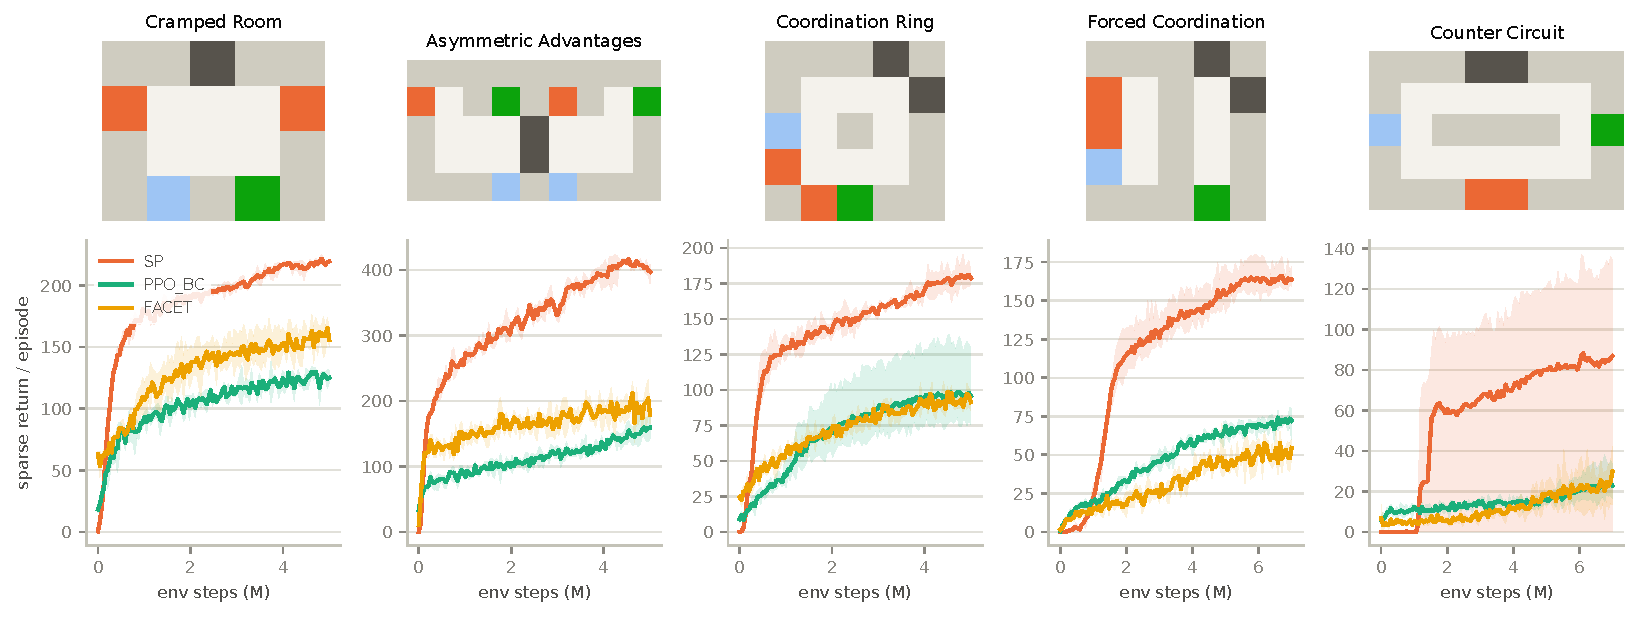
\includegraphics[width=\linewidth]{figs/layouts_curves.pdf}
\caption{\textbf{Top:} the five layouts (orange = onion dispensers, blue =
dish dispensers, dark = pots, green = serving windows). \textbf{Bottom:}
training curves (sparse return per episode; mean over 3 seeds, min--max
band). Curves are measured against each method's \emph{training} partners
and are not comparable across methods---SP plays with a copy of itself,
\ppobc{} with a stochastic human model, \facet{} with its mixed pool. One
SP seed on Counter Circuit never scored (flat 0 for 7M steps), a known
failure mode of self-play on this layout.}
\label{fig:layouts-curves}
\end{figure}

\paragraph{Self-play collapses when the partner changes.}
Table~\ref{tab:main} shows the classic result cleanly at our scale. SP
posts the highest self-paired scores everywhere (up to 406.0 on Asymmetric
Advantages) yet drops 53\% (Cramped Room), 79\% (Coordination Ring), 85\%
(Asymmetric Advantages), 86\% (Counter Circuit), and 96\% (Forced
Coordination) when moved to held-out human proxies. On Forced
Coordination---where neither player can complete a soup alone---SP with a
human proxy (5.8) is \emph{worse than plain BC} (8.2), reproducing
\citet{carroll2019utility}'s central observation that self-paired
performance is not predictive of human-paired performance.

\paragraph{Human anchoring is the single strongest ingredient.}
\ppobc{} is the best human-proxy method on three of five layouts
(Asymmetric Advantages 136.9, Coordination Ring 57.6, Forced Coordination
39.1) and ties SP on Cramped Room (102.7 vs.\ 103.3). At this compute
scale, concentrating all best-response capacity on a single human model
transfers to unseen human proxies better than spreading it across a
15-partner population: \ppobc{}'s mean exceeds \facet{}'s on four of five
layouts on this axis (on Cramped Room the 102.7-vs-90.2 gap is within
\facet{}'s seed s.e.\ of $\pm$18.6), though \facet{} clearly beats SP
where SP collapses hardest (84.4 vs.\ 60.0 on Asymmetric Advantages;
35.3 vs.\ 5.8 on Forced Coordination) and trails \ppobc{} on Forced
Coordination by less than the sum of their s.e.s. Counter Circuit is
sobering for every RL method: BC itself (17.6) is the top proxy-paired
policy, echoing the original paper's finding on this layout.

\paragraph{Specialists pay on the other axis.}
Table~\ref{tab:fleet} completes the picture. \ppobc{}'s human
specialization costs it with machine partners: 136.4 vs.\ \facet{}'s 203.6
on Cramped Room, 82.2 vs.\ 132.2 on Forced Coordination, 13.8 vs.\ 36.7 on
Counter Circuit. The specialization runs deep enough that \ppobc{} is not
even compatible with \emph{itself}: two copies of the same \ppobc{} agent
score 0.0 on Cramped Room and Counter Circuit (Table~\ref{tab:main},
\emph{with self} rows) while the same agents score 102.7 and 5.3 with human
proxies---both copies occupy the role the human model used to fill, a
concrete instance of the cooperative incompatibility studied by
\citet{li2023cooperative}. We verified this is genuine deadlock rather than
inactivity: the agents move and interact throughout the episode without
ever completing a delivery chain. Importantly, \emph{\facet{} exhibits the
same failure}: its self-pairing scores 0.0 on Coordination Ring (all three
seeds), and its Cramped Room (70.7) and Counter Circuit (4.0) self-pair
means hide bimodal per-seed outcomes (212.0/0.0/0.0 and 0.0/12.0/0.0
respectively)---best-response training against any external partner
distribution, human or mixed, does not confer self-compatibility. Most
self-pair cells for both best-response methods are all-or-nothing per
seed, which the s.e.s in the \emph{with self} rows make visible. Cross-seed SP$+$SP pairing is strong where independent
runs converge to similar conventions (396.7 on Asymmetric Advantages) and
catastrophic where they do not (3.7 on Forced Coordination---a pure
convention clash, since each SP agent scores $\approx$160 with its own
copy). \facet{} is best or within one s.e.\ of best on four of five
layouts, with visibly lower seed variance in several cells
(141.3 $\pm$ 1.3 on Coordination Ring vs.\ 84.7 $\pm$ 23.2 for SP).

\paragraph{No catastrophic seed-averaged cells.}
Averaging the two axes per layout and then across layouts gives a combined
workspace-compatibility score of 110.3 for \facet{}, 102.0 for \ppobc{},
95.0 for SP, and 43.3 for BC (equal axis weighting; see
Section~\ref{sec:discussion}). More telling than the average is the
minimum: across all ten seed-averaged (layout $\times$ partner-type)
cells, \facet{}'s worst cell mean is 12.7, whereas SP bottoms out at 3.7,
\ppobc{} at 5.3, and BC at 5.8 (Figure~\ref{fig:gap} visualizes the
self-vs-proxy gaps). This is a property of 3-seed means, not of every
agent: \facet{}'s worst single seed scores 3.3 (Counter Circuit, seed 0,
with \hproxy{}; Appendix~\ref{app:perseed}), so individual \facet{} agents
can still fail, and three seeds is a thin basis for a robustness claim.
In a deployed workspace, the worst cell is the one users remember---and
seed selection against a validation partner would be part of any real
deployment.

\paragraph{The sampler finds the hard partners.}
Figure~\ref{fig:priority} tracks the prioritized sampler's probability
mass during \facet{} training. On the three easier layouts, mass
concentrates on the three BC human models (49--54\% of sampling, vs.\
20\% under uniform sampling)---the human models are the hardest partners
there. On Forced Coordination and Counter Circuit the mass shifts to the
early low-skill checkpoints instead: with an incompetent partner on these
layouts, no soup can be delivered at all, making those the
lowest-return partners. The prioritization thus adapts the curriculum per
layout without any manual tuning, at the cost of spending fewer samples on
the human models exactly on the layouts where human compatibility is
hardest---a plausible explanation for \facet{}'s remaining gap to
\ppobc{} on the human axis, and a concrete lever for future work.

\begin{figure}[t]
\centering
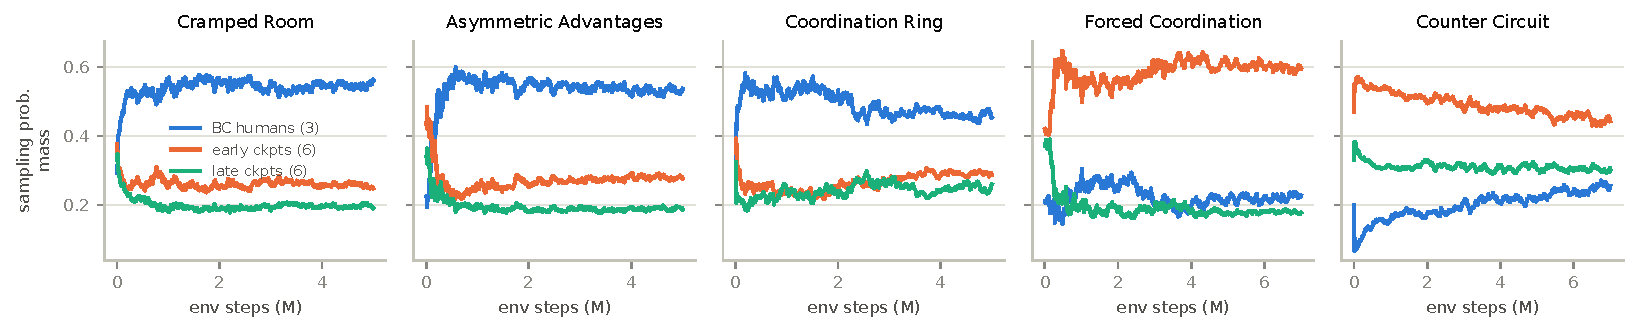
\includegraphics[width=\linewidth]{figs/priority.pdf}
\caption{Prioritized sampling mass over \facet{} training (seed 0), grouped
by partner type: BC human models (3 partners), early SP checkpoints
(8\%/20\%, 6 partners), late SP checkpoints (40\%/100\%, 6 partners).
The sampler concentrates on human models where they are the hardest
partners (left three layouts) and on low-skill checkpoints on the two
hard layouts.}
\label{fig:priority}
\end{figure}

\begin{figure}[t]
\centering
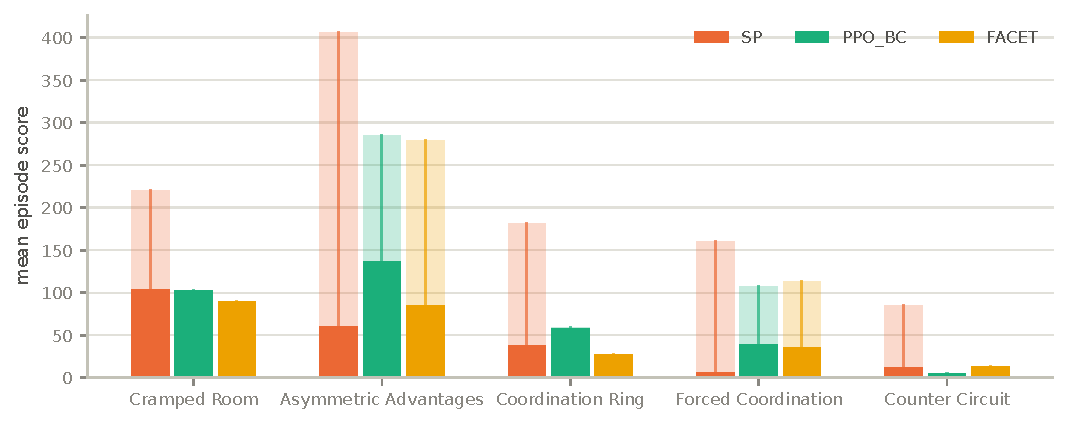
\includegraphics[width=0.9\linewidth]{figs/gap.pdf}
\caption{Self-paired score (pale) vs.\ score with held-out human proxies
(solid) for the three RL methods. The pale-to-solid drop is the
generalization gap that self-play maximizes and population/human-anchored
methods shrink.}
\label{fig:gap}
\end{figure}

\section{Discussion and Limitations}
\label{sec:discussion}

\paragraph{What the results support.}
Three conclusions are directly supported. First, the classic finding
reproduces at laptop scale: self-paired scores are never predictive of
human-paired scores, with drops of 53--96\%. Second, at this compute
scale human-data anchoring is the strongest single ingredient for the
human axis---\ppobc{} beats the population method on three of five
layouts, a useful negative result given that population methods dominate
recent literature at much larger scale~\citep{strouse2021collaborating,
zhao2023maximum}; our population is small (15 partners from 3 runs) and a
best response to it necessarily dilutes capacity relative to a
single-partner specialist. Third, specialization has a measurable price on
the other axis, and only the population method avoids catastrophic cells
across both axes. We would summarize the practical recipe for multiplayer
workspaces as: \emph{if you will only ever face humans, best-respond to a
human model; if you must coexist with a fleet as well, \facet{}-style
pools buy worst-case robustness for one extra PPO run.}

\paragraph{What the results do not support.}
Our results do not show that prioritized pools beat human-anchored best
response on the human axis at this scale---they do not, on three of five
layouts. We report this directly rather than aggregating it away; the
combined score (110.3 vs.\ 102.0) favors \facet{} only because the fleet
axis is weighted equally, which is a modeling choice about deployment,
not a finding.

\paragraph{Limitations.}
First, our human-side evaluation uses BC proxies, not live humans; proxy
evaluation is the field's standard first filter but is an imperfect
predictor of performance with real
humans~\citep{strouse2021collaborating,wang2024zsceval}, and a user study
remains future work. Second, all agents use the benchmark's
hand-designed featurization and old dynamics to remain commensurate with the
2019 human data; results may differ under pixel observations or the newer
dynamics. Third, our compute scale is deliberately small---one laptop---so
absolute scores trail large-scale reproductions; the comparisons are
internally controlled (identical architecture, budget, and evaluation for
every method), but ceilings may shift with more compute. Fourth,
Overcooked itself under-tests some coordination phenomena
\citep{gessler2025overcookedv2}; extending \facet{} to richer workspace
simulators---including the tool-use and approval-gate structure of real
enterprise workspaces---is the natural next step for Jewel Labs'
production setting. Fifth, our fleet axis is in-distribution for \facet{}
by construction---its pool contains the fleet agents' checkpoints,
including the final ones---so Table~\ref{tab:fleet} measures retained
compatibility with a known fleet, not zero-shot transfer to unknown
agents; a held-out-fleet evaluation (e.g., SP runs excluded from the pool)
would isolate the latter and we did not run one. Sixth, the released
browser demo replays each pairing's best episode from its best seed---it
is an illustration of learned behavior, not a random sample of the means
in Table~\ref{tab:main}. Finally, \facet{} inherits FCP's main cost: it
consumes the checkpoints of multiple self-play runs (plus a
$\sim$15--25\% per-step overhead for frozen-partner inference), though
the checkpoints are artifacts most practitioners already produce.

\section{Conclusion}
\label{sec:conclusion}

\facet{} is a deliberately minimal recipe---human-anchored population,
checkpoint skill diversity, worst-partner prioritization---trained and
evaluated end-to-end on a laptop across all five classic Overcooked
layouts. The study's clearest lessons are that self-play's 53--96\%
partner-transfer collapse survives every scale reduction; that a best
response to one behavior-cloned human remains the strongest pure
human-compatibility baseline at small scale; and that a prioritized pool
of human models plus self-play checkpoints is what removes the
catastrophic seed-averaged cells when agents must work with humans
\emph{and} a fleet that is known at training time---the defining
condition of a multiplayer workspace. For
organizations building such workspaces, the ingredients are already lying
around: behavior logs, self-play checkpoints, and a ten-line prioritized
sampler.

\subsubsection*{Acknowledgments}
We thank the Overcooked-AI authors for the benchmark, environment, and
human--human dataset~\citep{carroll2019utility}. Model training,
evaluation, and manuscript preparation used Claude (Anthropic) as an
engineering and drafting assistant; all experiments, numbers, and claims
were produced and verified by the pipeline released with this paper.

\bibliographystyle{plainnat}
\bibliography{refs}

\appendix

\section{Hyperparameters}
\label{app:hparams}

\begin{table}[h]
\centering
\caption{Complete hyperparameters. All methods share the PPO block; BC uses
the imitation block. No per-layout tuning was performed.}
\label{tab:hparams}
\small
\begin{tabular}{llll}
\toprule
\multicolumn{2}{l}{\textbf{PPO (SP, \ppobc{}, \facet{})}} &
\multicolumn{2}{l}{\textbf{Behavior cloning}} \\
\midrule
policy net & MLP $96{-}128{-}128{-}6$, $\tanh$ & net & MLP $96{-}64{-}64{-}6$, ReLU \\
value net & MLP $96{-}128{-}128{-}1$, $\tanh$ & optimizer & Adam, lr $10^{-3}$ \\
optimizer & Adam, lr $3{\times}10^{-4}$ & batch size & 512 \\
discount $\gamma$ / GAE $\lambda$ & 0.99 / 0.95 & max epochs & 60 \\
PPO clip & 0.2 & early stop & patience 8 (val.\ loss) \\
epochs $\times$ minibatch & $8\times2048$ & val.\ fraction & 0.1 \\
entropy coef. & $0.05\!\to\!0.005$ (80\%) & weight decay & $10^{-6}$ \\
value coef. / grad clip & 0.5 / 0.5 & & \\
reward scale & 0.1 & \multicolumn{2}{l}{\textbf{\facet{} population}} \\
shaped-reward anneal & $1\!\to\!0$ over 60\% & pool & 3 BC + 12 SP ckpts \\
parallel envs & 15 ($3\times5$), horizon 400 & ckpt stages & 8/20/40/100\% \\
steps (easy / hard layouts) & 5M / 7M & $\tau$, $\varepsilon$, EMA $\beta$ & 0.35, 0.25, 0.05 \\
\bottomrule
\end{tabular}
\end{table}

\section{Per-seed results}
\label{app:perseed}

\begin{table}[h]\centering\caption{Per-seed mean scores with \hproxy{} (30 episodes per seed: 3 proxy seeds $\times$ 10 episodes).}\label{tab:perseed}\small
\begin{tabular}{llccc}
\toprule
Layout & Method & seed 0 & seed 1 & seed 2 \\
\midrule
Cramped Room & BC & 60.7 & 62.0 & 54.0 \\
Cramped Room & SP & 106.7 & 93.3 & 110.0 \\
Cramped Room & PPO$_{\mathrm{BC}}$ & 108.0 & 99.3 & 100.7 \\
Cramped Room & \facet{} & 127.3 & 71.3 & 72.0 \\
Asymm.\ Advantages & BC & 75.3 & 70.0 & 59.3 \\
Asymm.\ Advantages & SP & 73.3 & 62.0 & 44.7 \\
Asymm.\ Advantages & PPO$_{\mathrm{BC}}$ & 107.3 & 138.0 & 165.3 \\
Asymm.\ Advantages & \facet{} & 96.7 & 77.3 & 79.3 \\
Coordination Ring & BC & 24.0 & 19.3 & 22.0 \\
Coordination Ring & SP & 34.7 & 40.0 & 38.0 \\
Coordination Ring & PPO$_{\mathrm{BC}}$ & 30.7 & 22.7 & 119.3 \\
Coordination Ring & \facet{} & 25.3 & 23.3 & 33.3 \\
Forced Coordination & BC & 6.7 & 7.3 & 10.7 \\
Forced Coordination & SP & 0.7 & 14.7 & 2.0 \\
Forced Coordination & PPO$_{\mathrm{BC}}$ & 38.0 & 43.3 & 36.0 \\
Forced Coordination & \facet{} & 38.7 & 34.0 & 33.3 \\
Counter Circuit & BC & 16.0 & 17.3 & 19.3 \\
Counter Circuit & SP & 0.0 & 22.0 & 14.0 \\
Counter Circuit & PPO$_{\mathrm{BC}}$ & 7.3 & 2.7 & 6.0 \\
Counter Circuit & \facet{} & 3.3 & 22.0 & 12.7 \\
\bottomrule
\end{tabular}\end{table}

\section{Reproducibility}
\label{app:repro}

All experiments are reproducible from the released repository:
\texttt{python -m facet.data} and \texttt{python -m facet.bc} build the
datasets and BC models ($\sim$25 minutes);
\texttt{scripts/run\_batch.sh} executes the PPO stages via
\texttt{scripts/queue\_sp.txt} then \texttt{scripts/queue\_br.txt}
($\sim$5 hours on a 10-core M4; the queue files carry the paper's
step/worker settings---\texttt{train\_ppo.py}'s bare defaults are
smaller); \texttt{scripts/evaluate.py} and \texttt{scripts/eval\_fleet.py}
produce the raw episode scores per layout; and
\texttt{scripts/analyze.py} (\texttt{results}, \texttt{fleet},
\texttt{figures}) regenerates every table and figure from them. Random
seeds are fixed (0, 1, 2) at every stage.

\end{document}
